\documentclass[conference]{IEEEtran}
\IEEEoverridecommandlockouts
\usepackage{cite}
\usepackage{amsmath,amssymb,amsfonts}
\usepackage{graphicx}
\usepackage{booktabs}
\usepackage{multirow}
\usepackage{url}
\usepackage{xcolor}
\usepackage{pgfplots}
\pgfplotsset{compat=1.18}
\usepackage[hidelinks]{hyperref}

% FIRST DRAFT 2026-11-18. Red text = pending result or a decision for the team.
\newcommand{\todo}[1]{\textcolor{red}{[#1]}}
\newcommand{\sig}{$^{*}$}

\begin{document}

\title{How Much Lookahead Does Learned Video Rate Control Need?\\ Per-Frame, Per-Stream and Live-Channel Results on x264 and x265}

\author{\IEEEauthorblockN{Aayush Soni, Ahhana Gupta, Atharva Kulkarni, Pavneet Singh Banga, Sara Pirasteh}
\IEEEauthorblockA{EE599 Reinforcement Learning, University of Southern California, Los Angeles, CA, USA}}

\maketitle

\begin{abstract}
A video encoder must choose a quantization parameter (QP) for every frame so that a segment fits a bit budget at the best possible quality. An offline search that sees a whole group of pictures (GOP) and tries hundreds of real encodes finds much better QP plans than any single-pass controller, but it cannot run live. We ask how much of that gain a single-pass policy can recover, how this changes with the lookahead $k$ (the number of future frames whose first-pass cost the policy may see), and where reinforcement learning (RL) helps beyond a well-tuned hand-designed controller. All results use one dataset (109 clips, 1{,}042 GOPs, split by source), real x264 and x265 encodes, budgets and initial QPs that use only information available at decision time, one quality-at-budget metric in dB, and confidence intervals clustered by source. Inside a GOP, lookahead pays off early: a tuned causal controller gains about 0.2~dB from $k{=}0$ to $k{=}2$ and nothing beyond $k{=}5$. A residual PPO policy started from imitation of the search beats this controller on held-out test clips by $+0.07$~dB (x264) and $+0.16$~dB (x265), replicates on a second, fresh test set of 93 unseen clips ($+0.04$ / $+0.19$~dB), and halves its over-budget rate; neither imitation alone nor RL alone beats it. When several GOPs share one budget without a network, a rule tuned for single-clip streams matches RL on them but loses 0.3~dB on mixed streams, a rule tuned for all streams does the reverse, and RL beats each where it is weak. When the bits must also cross a time-varying channel with a latency cap, imitation of a hindsight oracle followed by PPO beats tuned buffer rules by 0.25--0.66~dB, including 0.12--0.24~dB on single-clip streams, with fewer stalls, and the gain holds in VMAF (+1.1 to +2.8 points at 1080p); it does not, however, beat the encoder's own whole-stream ABR+VBV with a tuned target, which ties it in most settings and wins in one. RL helps where the decision has a long horizon and a hard-to-model state (buffer, channel, mixed content); it does not help where a tuned rule already captures the structure.
\end{abstract}

\begin{IEEEkeywords}
video coding, rate control, x264, x265, reinforcement learning, imitation learning, constrained RL, live streaming
\end{IEEEkeywords}

%=====================================================================
\section{Introduction}
%=====================================================================
Rate control decides how many bits each frame receives. A lower QP spends more bits for higher fidelity, and because frames are predicted from one another, bits spent early improve the references of later frames~\cite{sullivan1998rdo,ortega1998rd}. Production encoders use hand-designed rate models and, when delay allows, a lookahead buffer that analyses upcoming frames with a fast first pass~\cite{garrett2009mbtree,x264,x265,li2014lambda}. Lookahead costs latency: at 30~fps every frame of lookahead is 33~ms. A live encoder designer must decide how much delay to pay for, and this is usually decided by experience rather than measurement.

Our research question, fixed in the proposal, is: \emph{how much of a hindsight search's gain can a single-pass policy capture, and how does that change with the number of future frames it may see?} We study it at three levels of the rate-control problem:
\begin{enumerate}
\item \textbf{Per frame, inside one GOP} (the proposal's setting): a fixed GOP budget, lookahead $k\in\{0,2,5,10,29\}$.
\item \textbf{Per GOP, inside a stream}: several GOPs share one budget, the setting of on-demand encoding.
\item \textbf{Per GOP, through a live channel}: the bits leave through a time-varying channel and a sender buffer with a latency cap, where a stall is the dominant cost.
\end{enumerate}

Our contributions are: (i) a controlled measurement of the value of lookahead under a fixed budget, with budgets and initialization that use only information available at decision time; (ii) a decomposition showing that the gain of the best learned controller comes from imitation of the search \emph{and} RL fine-tuning together; (iii) a map of where RL helps and where a tuned rule is enough, across the three levels; (iv) separate reporting of quality and budget violations, with the scene detector's own lookahead counted as delay; and (v) negative results, reported with the same statistics as the positive ones.

%=====================================================================
\section{Motivation and Related Work}
%=====================================================================
\textbf{Classical rate control.} Model-based controllers fit a rate model (e.g.\ the $R$--$\lambda$ model of HEVC~\cite{li2014lambda}) and allocate bits by frame type and complexity~\cite{chen2007rcsurvey}. x264's MB-tree and x265's CU-tree propagate the importance of reference blocks over a lookahead window~\cite{garrett2009mbtree}. Single-pass ABR with a VBV buffer is the standard live mode; two-pass encoding sees the whole clip.

\textbf{Learned rate control.} RL has been applied to HEVC intra-frame rate control~\cite{hu2018rlintra}. Closest to our work are two lines from VP9/libvpx two-pass encoding. Mao~\emph{et~al.}~\cite{mao2020neural} learn a rate-control policy by imitating the plans of an offline search, prune spurious actions at inference, and add feedback control to hit the target bitrate. Mandhane~\emph{et~al.}~\cite{mandhane2022muzero} train a MuZero agent~\cite{schrittwieser2020muzero} with self-competition to optimise quality under a bitrate constraint. Both show that search-based learning beats the default controller in a two-pass setting. We differ in three ways that follow the feedback on our proposal: we control the \emph{lookahead} explicitly and measure its value, from strictly causal to the whole GOP; we separate what imitation of the search gives from what additional RL interaction gives; and we analyse GOPs with scene cuts separately from stable ones.

\textbf{Adaptive streaming.} Choosing a bitrate per segment over a network is the adaptive bitrate (ABR) problem. Buffer-based rules (BOLA~\cite{spiteri2016bola}), model-predictive control~\cite{yin2015mpc}, and RL (Pensieve~\cite{mao2017pensieve}) are the standard approaches. Puffer showed that a learned throughput predictor helps in the wild~\cite{yan2020puffer}. Our live-channel setting borrows the channel and buffer model and the MPC baseline from this line, but the decision is the encoder's QP, not a choice among pre-encoded renditions.

\textbf{RL tools we use.} PPO~\cite{schulman2017ppo}; behaviour cloning and DAgger~\cite{pomerleau1989alvinn,ross2011dagger}; offline RL (CQL~\cite{kumar2020cql}); constrained RL via Lagrangian and PID-Lagrangian multipliers~\cite{altman1999cmdp,tessler2019rcpo,stooke2020pid}; residual policies on a base controller~\cite{silver2018residual,johannink2019residual}; and asymmetric actor-critic with a privileged critic~\cite{pinto2018asymmetric}.

%=====================================================================
\section{Problem Formulation and Theory}
%=====================================================================
\subsection{Per-frame control inside a GOP}
An episode is one GOP of $T{=}30$ frames (one IDR frame and 29 P frames) with budget $B$. At frame $t$ the policy sees the bits spent so far, the budget left, its recent QPs and outcomes, the first-pass cost of frame $t$, and the first-pass cost of the next $k$ frames. It outputs QP$_t$; the real encoder codes the frame. The episode is scored once, at its end:
\begin{equation}
S = \Delta\mathrm{PSNR}_B - 0.17\cdot \max\!\Big(0,\,100\tfrac{R-B}{B}\Big),
\end{equation}
where $R$ is the GOP's bits and $\Delta\mathrm{PSNR}_B$ is the PSNR minus the PSNR of the constant QP that spends exactly $B$ (from the GOP's constant-QP curve, QP 18--50). $S{=}0$ means ``as good as the best constant QP chosen in hindsight''. The price of 0.17~dB per 1\% over is about the slope of PSNR in rate near the operating point, so overspending is never free. Unused budget is not rewarded.

\textbf{What may be known at decision time.} A budget computed from the GOP's own encode tells the controller how expensive the GOP is, and an initial QP that meets such a budget is an oracle. Both are removed. The budget at level $q_0\in\{24,30,36,42\}$ is the clip's mean constant-QP bits per GOP at $q_0$: what a two-pass encoder knows after its first pass; the GOP enters it only as one of the clip's GOPs, never through its own cost alone. The controller's starting QP comes from a causal rate model of frame 0, the visible first-pass costs and the previous GOP's outcome. Scene-cut flags use only visible frames.

\textbf{Residual control.} The base is a tuned causal controller (``the controller''): a rate model updated online that sets the next QP from the budget left and the visible costs, with the previous GOP's outcome as a prior. A residual policy adds an integer offset in $[-6,6]$ to the controller's real-valued QP, with a per-position mean shift learned from the search plans and a hard bit cap. This keeps the learner on the budget at $k{=}0$, where a QP-only action cannot find the right level.

\textbf{Imitation, then RL.} The hindsight search (a hill-climb over QP plans with about 600 real encodes per GOP and budget) provides labels. Behaviour cloning (BC) of those plans suffers covariate shift: once the cloned policy drifts, it reaches states the search never visited~\cite{ross2011dagger}. PPO from the BC policy corrects the drift with the true closed-loop return. We train the critic alone for the first 20k steps so the BC actor is not destroyed by early random advantages.

\textbf{Detector delay.} A controller that requests extra lookahead only near scene cuts needs a detector that knows a cut lies inside the next $K$ frames. At every frame this detector must have read $\min(K, T{-}1{-}t)$ frames ahead, plus 2 frames to reject flashes. Averaged over a 30-frame GOP this is 1.9 (3.7) frames for $K{=}2$, 4.5 (6.1) for $K{=}5$ and 8.2 (9.4) for $K{=}10$, without (with) flash rejection. That is the true encoding delay of a cut-triggered mode, not the number of frames the controller's features cover.

\subsection{Per-GOP control inside a stream}
A stream of $n$ GOPs has one budget $B = s\sum_g B_g$, with level $q_0$ and scale $s\in\{0.85,1,1.18\}$ never observed. Each step chooses one GOP's constant QP as an offset in $[-6,6]$ on a causal model QP; outcomes come from the measured constant-QP curves. The score is (1) on the stream's pooled PSNR. The baseline is a remaining-budget rule (spend the remaining budget in proportion to predicted cost, with a margin and a prior weight).

\subsection{Live channel with a latency cap}
The bits now leave through a channel. GOP $i$ (1~s) drains at rate $R_i = m_i\,\bar r$, where $\bar r = B/n$ and $\log m_i$ follows an AR(1) process ($\rho{=}0.8$, $\sigma{=}0.3$) or a real 4G/LTE throughput trace~\cite{vanderhooft2016lte}, observed after the GOP. The sender buffer holds at most 1~s at the mean rate; anything above stalls playback for excess$/R_i$ seconds. The score subtracts 0.5~dB per 1\% of duration stalled from (1). Since $\bar r$ follows from $B$, a budget derived from the stream's own clips would tell every controller how expensive the stream is. A live encoder has no first pass, so here the budget comes from a fixed bitrate ladder: $B = s\, n\, L(q_0)$, where $L(q_0)$ is the median over \emph{training} GOPs of constant-QP bits per GOP at $q_0$, the same for every stream. The base rule, \textbf{vbv2}, sets a target from the rate estimate shrunk by observed volatility plus a buffer-tracking term and an optional remaining-budget clamp (5 parameters tuned on validation over a wide grid). \textbf{MPC} adds offsets chosen by simulating the buffer over $H$ GOPs on 64 sampled channel paths with the true channel model~\cite{yin2015mpc}. \textbf{ppo\_v2} is PPO acting as a residual on vbv2. \textbf{il\_ppo} first imitates a hindsight oracle (a dynamic program that knows the future channel and content) with DAgger, then fine-tunes with PPO.

%=====================================================================
\section{Experimental Setup}
%=====================================================================
\textbf{Data.} 109 clips at $320{\times}180$, 8-bit 4:2:0, from Blender open movies~\cite{blender}, Xiph~\cite{xiph}, UVG~\cite{mercat2020uvg} and YouTube UGC~\cite{wang2019ugc}; 1{,}042 full 30-frame GOPs. Splits are by source group (film, shoot or uploader): 66/16/27 clips (625/152/265 GOPs) for train/validation/test. Scene cuts were labelled by two detectors with manual review of every disagreement (89/110 exact agreement with a second human reviewer). Test has 211 stable, 49 cut and 5 gradual GOPs. A second test set, \emph{test2}, was built and pre-registered after the first test pass and is used only for evaluation: 93 YouTube UGC clips in 12 categories, one per uploader and no uploader shared with the first set, 860 scored GOPs, labelled with the same protocol. Three first-set clips run through the test2 code path reproduce every stored row exactly.

\textbf{Encoders.} x264 0.165 and x265 4.1, preset medium, IPPP, keyint 30, scene-cut detection, AQ, MB-tree/CU-tree and psy off, one thread, QPs forced per frame. All bits and PSNRs come from real encodes; stream and live levels look up the measured per-GOP constant-QP curves, and we verify by re-encoding that the lookups equal real encodes exactly. Quality is 6:1:1 YUV PSNR averaged over frames at the per-GOP level and luma PSNR of pooled MSE at the stream and live levels, each plane capped at 100~dB.

\textbf{Protocol.} Selection on a fold of the training clips, confirmation on validation, and a single pre-registered test pass for the per-GOP headline. Every method is rescored with one metric function on the same curves and budgets. Differences are paired on the same (GOP or stream, level, $k$) and reported with 95\% bootstrap intervals over source groups~\cite{efron1993bootstrap}; a spliced stream is its own cluster. ${}^{*}$ marks an interval that excludes 0. Learners use 3 seeds, averaged per case. Budget level 24 episodes whose budget exceeds the GOP's QP-18 spend are excluded from the per-GOP primary analysis. Primary comparisons were fixed before the results (R3 vs.\ the controller; RL vs.\ the re-tuned rule on single-clip streams; ppo\_v2 and il\_ppo vs.\ vbv2); the many other intervals are descriptive and not corrected for multiple comparisons. The proposal also listed A2C, DQN and a safety shield. On this dataset we compare BC, CQL$\to$PPO, residual PPO, Lagrangian and PID-Lagrangian PPO, a recurrent policy (stream level) and oracle imitation; a budget shield lowered every method's score in a preliminary test and was dropped.

\textbf{Baselines.} Constant QP at the matching QP (the zero of the metric); the encoders' own single-pass ABR with VBV sized to the budget and \texttt{--rc-lookahead} $k$, with a target margin tuned on validation; two-pass (stream level only, non-causal); the tuned causal controller; and the hindsight search (not deployable, the ceiling).

%=====================================================================
\section{Results}
%=====================================================================
\subsection{Per-frame control: the value of lookahead}
Table~\ref{tab:kcurve} gives the test score by lookahead. Three facts stand out. First, \textbf{no single-pass method reaches the search}: the search scores $+0.30$/$+0.28$~dB (x264/x265), while the controller stays 0.12--0.28~dB below constant QP at $k\ge 2$. Second, \textbf{lookahead's value is front-loaded}: the controller gains $+0.19$/$+0.16$~dB from $k{=}0$ to $k{=}2$, $+0.03$/$+0.07$ from $k{=}2$ to $k{=}5$, and nothing beyond (the whole GOP is slightly worse than $k{=}5$). About 2--5 frames (67--167~ms) buy all of it. In the proposal's terms (lower block of Table~\ref{tab:kcurve}), a single-pass controller captures about two thirds of the search's gain over the encoder's own rate control with no lookahead (66\%/52\%), about three quarters with 2--5 frames (75--77\% / 62--67\%), and no more with the whole GOP; R3 raises this to 81\%/79\% at $k{=}5$. Knowing the previous GOP's outcome substitutes for delay at $k{=}0$ ($+0.14$~dB [$+0.03$, $+0.24$] on x264). Third, \textbf{the encoders' own ABR+VBV is far behind} ($-1.2$ to $-1.7$~dB at every $k$, over budget on half or more of the GOPs) and does not improve with lookahead.

\begin{table}[t]
\caption{Per-GOP test score $S$ (dB) by lookahead $k$, clip-level (two-pass) budgets. 0 = best constant QP in hindsight. Lower block: share of the search's gain over the encoder's ABR+VBV that each method captures, $(S-S_{\mathrm{ABR}})/(S_{\mathrm{search}}-S_{\mathrm{ABR}})$, with $S_{\mathrm{ABR}}$ at the middle of its range ($\pm1$ point). Learners: 3 seeds. Budget-level-24 episodes beyond the QP-18 spend included.}
\label{tab:kcurve}
\centering\footnotesize\setlength{\tabcolsep}{3.2pt}
\resizebox{\columnwidth}{!}{\begin{tabular}{@{}lccccc|ccccc@{}}
\toprule
& \multicolumn{5}{c|}{x264} & \multicolumn{5}{c}{x265}\\
$k$ & 0 & 2 & 5 & 10 & 29 & 0 & 2 & 5 & 10 & 29\\
\midrule
Search (ceiling) & \multicolumn{5}{c|}{$+0.30$} & \multicolumn{5}{c}{$+0.28$}\\
Controller & $-.35$ & $-.16$ & $-.13$ & $-.12$ & $-.13$ & $-.43$ & $-.28$ & $-.21$ & $-.19$ & $-.24$\\
BC (causal base) & $-1.49$ & $-.85$ & $-.56$ & $-.41$ & $-.20$ & $-1.37$ & $-.88$ & $-.60$ & $-.40$ & $-.21$\\
CQL$\to$PPO & $-1.27$ & $-.76$ & $-.58$ & $-.42$ & $-.37$ & $-1.12$ & $-.78$ & $-.53$ & $-.43$ & $-.41$\\
ABR+VBV & \multicolumn{5}{c|}{$-1.52$ to $-1.64$} & \multicolumn{5}{c}{$-1.16$ to $-1.25$}\\
\midrule
\multicolumn{11}{@{}l}{\emph{Share of the search's gain captured (\%)}}\\
Controller & 66 & 75 & 77 & 78 & 77 & 52 & 62 & 67 & 68 & 65\\
R3 & & & 81 & & & & & 78 & & \\
BC (causal base) & 5 & 39 & 54 & 62 & 73 & $-11$ & 22 & 41 & 54 & 67\\
CQL$\to$PPO & 16 & 44 & 53 & 62 & 64 & 6 & 28 & 45 & 52 & 54\\
\bottomrule
\end{tabular}}
\end{table}

\subsection{Per-frame control: where RL beats the controller}
Learners that set the QP from a learned base (BC, CQL$\to$PPO) never pass the controller (Table~\ref{tab:kcurve}): their large $k$-curves are mostly budget repair. A plain residual PPO on the controller also ends below it. The method that wins (R3) combines three parts: the controller as the base, a BC actor trained on the search plans (labels centred on the controller), and PPO at the metric's price ($\lambda{=}0.17$, 180k steps, 20k critic-only warm-up).

\begin{table}[t]
\caption{R3 (imitation start + residual PPO on the controller) at $k{=}5$, clip-level (two-pass) budgets, dB. Test: single pre-registered pass on the first test set (27 clips). Test2: 93 fresh clips, pre-registered, evaluation only. 95\% CI over clips (source groups).}
\label{tab:r3}
\centering\footnotesize\setlength{\tabcolsep}{2.4pt}
\resizebox{\columnwidth}{!}{\begin{tabular}{@{}lcccc@{}}
\toprule
& \multicolumn{2}{c}{x264} & \multicolumn{2}{c}{x265}\\
& test & test2 & test & test2\\
\midrule
R3 $-$ controller (primary) & $+0.067$\sig & $+0.044$\sig & $+0.163$\sig & $+0.187$\sig\\
\quad 95\% CI & [$+.023$, $+.107$] & [$+.008$, $+.082$] & [$+.086$, $+.243$] & [$+.138$, $+.235$]\\
\quad stable GOPs & $+0.069$\sig & $+0.051$\sig & $+0.179$\sig & $+0.192$\sig\\
\quad cut / gradual GOPs & $+0.060$ & $-0.036$ & $+0.102$ & $+0.133$\sig\\
\quad R3 fed its own history & $+0.071$\sig & $+0.036$ & $+0.151$\sig & $+0.184$\sig\\
R3 $-$ controller, $k{=}2$ & -- & $+0.031$ & -- & $+0.146$\sig\\
R3 $-$ controller, $k{=}0$ / $k{=}29$ & -- & $+0.097$\sig / $+0.032$\sig & -- & --\\
R3 $-$ BC alone & -- & $+0.203$\sig & -- & $+0.207$\sig\\
R3 $-$ CQL$\to$PPO (540k steps) & $+0.129$\sig & $+0.305$\sig & $+0.199$\sig & $+0.304$\sig\\
R3 $-$ encoder ABR+VBV & $+1.047$\sig & $+2.239$\sig & $+0.711$\sig & $+1.518$\sig\\
\midrule
Quality at the bits: R3 / contr. & $+.130$ / $+.067$ & -- & $+.120$ / $-.030$ & --\\
GOPs over budget: R3 / contr. & 24 / 55\% & 25 / 53\% & 21 / 55\% & 20 / 55\%\\
\bottomrule
\end{tabular}}
\end{table}

Table~\ref{tab:r3} reports quality and budget violations separately, as the milestone feedback asked. R3 gains on both: it spends the bits better (higher quality for the bits it uses) and goes over budget less than half as often, landing slightly under budget ($-1.5$\% signed spend error), which costs less than going over. The gain is largest at the tightest budget on x265 ($+0.40$~dB at level 42).

\textbf{Replication on fresh clips.} Nothing was trained, refit or tuned on test2. R3 beats the controller there on both encoders, with every seed positive (Table~\ref{tab:r3}, Fig.~\ref{fig:test2}). On x265 the gain is broad: stable and cut GOPs, $k{=}2$ and $k{=}5$, and 10 of 12 content categories. On x264 it is smaller and comes from stable GOPs; the cut slice is not significant on either test set, so we do not claim that RL handles cuts better. R3 models trained at $k{=}0$ and $k{=}29$ (x264 only) also beat the controller on test2, by most at $k{=}0$, where the controller is weakest. Neither gains more from extra lookahead than the controller does. Running R3 on its own previous-GOP outcome instead of the controller's changes the score by less than 0.01~dB. Two sensitivity checks: training from 60k to 180k steps raises the validation gain ($+0.03\to+0.08$ / $+0.15\to+0.21$) and 360k adds nothing; rescoring the sealed test rows at other overshoot prices keeps R3 ahead on x265 at every price from 0 to 0.68~dB per \%, while on x264 its edge vanishes when overshoot is free ($+0.01$ at price 0).

\begin{figure}[t]
\centering
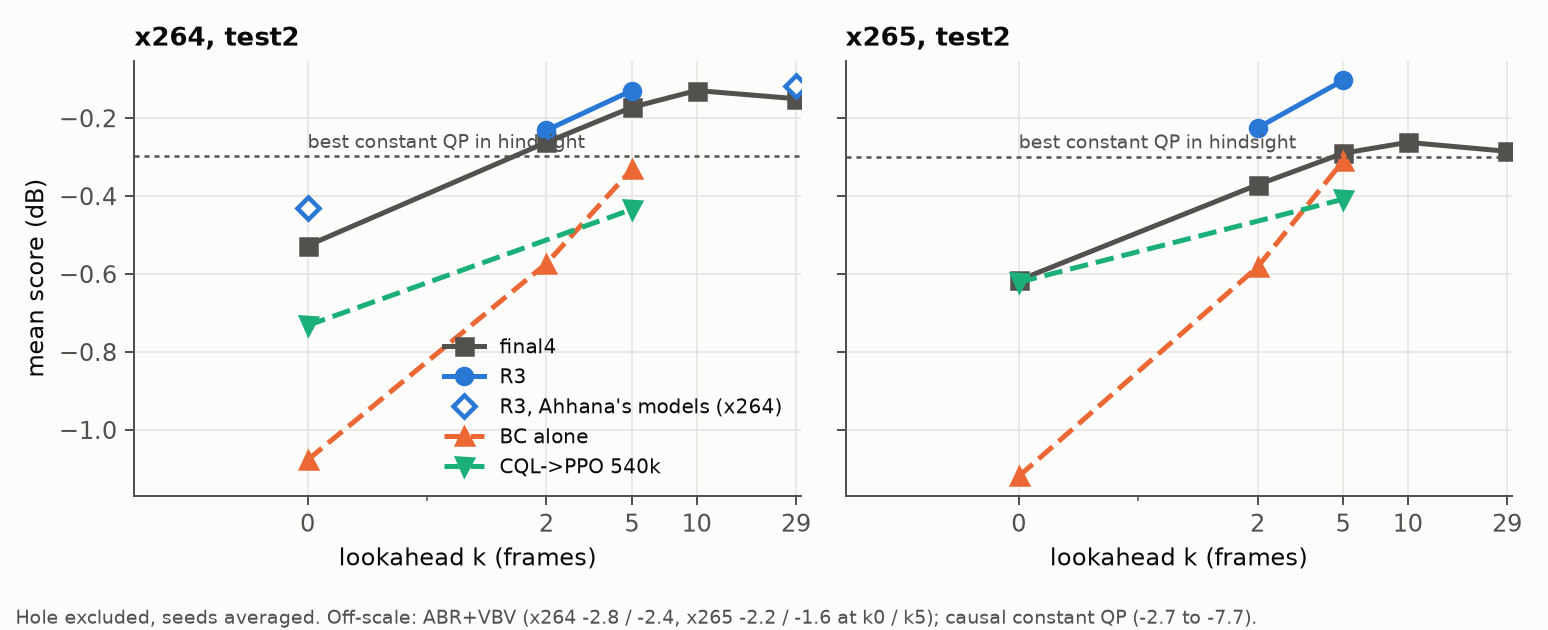
\includegraphics[width=\columnwidth]{figs/fig2_test2_kcurve.png}
\caption{Score by lookahead on test2 (fresh clips; ``final4'' = the controller). Open diamonds: R3 trained at $k{=}0$ and $k{=}29$ (x264). Off-scale: ABR+VBV ($-1.6$ to $-2.8$).}
\label{fig:test2}
\end{figure}

\begin{figure}[t]
\centering
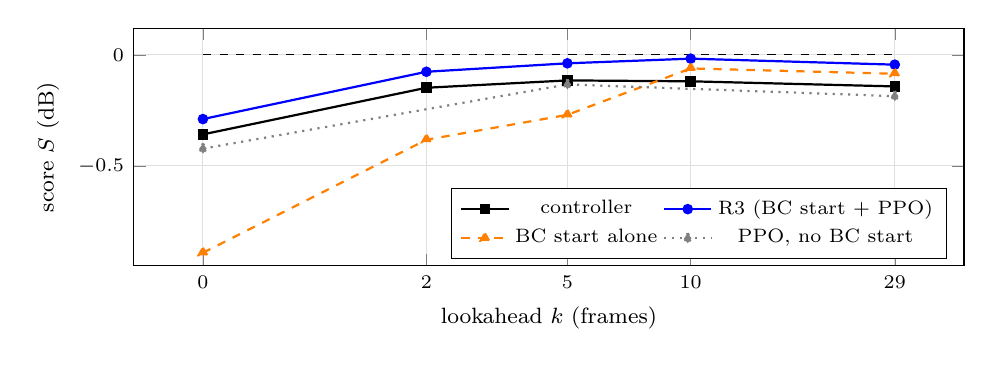
\begin{tikzpicture}
\begin{axis}[width=\columnwidth, height=4.6cm, xlabel={lookahead $k$ (frames)}, ylabel={score $S$ (dB)},
  xmode=log, log basis x=2, xtick={1,3,6,11,30}, xticklabels={0,2,5,10,29},
  ymin=-0.95, ymax=0.12, legend style={font=\scriptsize, at={(0.98,0.03)}, anchor=south east, legend columns=2},
  tick label style={font=\scriptsize}, label style={font=\footnotesize}, grid=major, grid style={gray!25}]
\addplot[black, thick, mark=square*, mark size=1.5pt] coordinates {(1,-0.358) (3,-0.148) (6,-0.115) (11,-0.119) (30,-0.142)};
\addlegendentry{controller}
\addplot[blue, thick, mark=*, mark size=1.5pt] coordinates {(1,-0.289) (3,-0.076) (6,-0.038) (11,-0.017) (30,-0.044)};
\addlegendentry{R3 (BC start + PPO)}
\addplot[orange, thick, dashed, mark=triangle*, mark size=1.8pt] coordinates {(1,-0.891) (3,-0.382) (6,-0.270) (11,-0.061) (30,-0.085)};
\addlegendentry{BC start alone}
\addplot[gray, thick, dotted, mark=diamond*, mark size=1.8pt] coordinates {(1,-0.422) (6,-0.133) (30,-0.186)};
\addlegendentry{PPO, no BC start}
\addplot[black, dashed, domain=1:30, samples=2, forget plot] {0};
\end{axis}
\end{tikzpicture}
\caption{Lookahead curve on validation (x264). R3 beats the controller by $+0.07$ to $+0.10$~dB at every $k$ (all CIs above 0). The BC start alone drifts at small $k$; PPO without it never beats the controller.}
\label{fig:kcurve}
\end{figure}

\textbf{Imitation alone vs.\ imitation followed by RL.} Fig.~\ref{fig:kcurve} (validation, x264) answers the proposal reviewer's question of whether RL interaction adds anything beyond imitating the search. It does, but only together with the imitation start:
\begin{itemize}
\item \emph{BC alone} loses badly at small $k$ ($-0.53$~dB vs.\ the controller at $k{=}0$) because of closed-loop drift, and reaches the controller only at $k\ge10$.
\item \emph{PPO without the BC start} never beats the controller at any $k$ ($-0.06$, $-0.02$, $-0.04$ at $k{=}0,5,29$).
\item \emph{R3 minus the same PPO from the standard start} is $+0.13$, $+0.10$, $+0.14$~dB at $k{=}0,5,29$, all significant.
\end{itemize}
At small $k$ PPO mostly repairs a poor imitation start; at large $k$ the start is already good and PPO polishes it. Absolute quality still levels off at $k\approx5$--10, so the learned controller does not change the lookahead answer.

\textbf{Scene cuts and adaptive lookahead.} The search changes QP around a cut in a characteristic way: $+0.5$ on the frame before the cut and $-0.7$ on the cut frame, and about 47\% of its QP change around cuts happens \emph{before} the cut, so it needs lookahead. For the controller, lookahead is worth about twice as much on cut GOPs ($k{=}5$ minus $k{=}0$: $+0.38$~dB) as on stable ones ($+0.18$; difference $+0.20$ [$+0.04$, $+0.39$] on x264). This suggests requesting lookahead only around cuts. With the class known in hindsight, $k{=}2$ on stable and $k{=}5$ on cut GOPs (mean 2.6 frames) is 0.02--0.05~dB below fixed $k{=}5$. Counting the detector's own scan makes it worse: to know whether a cut lies within the next 5 frames, a causal detector reads 4.5 frames ahead on average (6.1 with flash rejection), as many as fixed $k{=}5$. \textbf{Cut-triggered lookahead saves no delay here.} A gate that runs the best learner only around cuts gains at most $+0.01$~dB.

\subsection{Several GOPs sharing one budget}
Table~\ref{tab:stream} summarises the stream level (8-GOP streams, no network). We report two tunings of the remaining-budget rule, both on validation, that differ only in the streams they were tuned on. \emph{Rule A} is tuned on single-clip streams, the pre-registered primary population: its prior weight goes to almost zero, so it calibrates its rate model on the stream's own coded GOPs, and it plans to spend the whole budget. \emph{Rule B} is tuned on all streams: its prior counts as 3--6 GOPs and it keeps a 2\% margin. Against rule A the primary comparison fails: \textbf{RL does not beat a rule tuned for single-clip streams on single-clip streams}. Against rule B, RL is ahead there too ($+0.05$ / $+0.13$\sig, x264 / x265 throughout). Rule A is better on single-clip streams ($+0.10$ / $+0.09$ on test, n.s.; $+0.15$ / $+0.17$ on validation) because inside one clip the first GOPs predict the rest; on mixed streams the same choice misleads it, so it overspends on 34 / 24\% of streams (rule B 14 / 14\%) and scores 0.26--0.38~dB lower. With the content-blind ladder budget its single-clip edge shrinks to $+0.05$ / $+0.02$, while its mixed-stream loss stays. No rule setting wins on both, and RL beats each rule where it is weak: on mixed streams by $+0.60$ / $+0.55$ over rule A and $+0.22$ / $+0.33$ over rule B. PID-Lagrangian PPO~\cite{stooke2020pid} reaches a chosen over-budget rate by itself ($\lambda\approx0.36$--0.48, close to a hand-picked 0.34) and beats rule B at equal reliability. Lookahead over future GOPs is worth about $+0.25$~dB in PSNR for rule B and RL alike (but see the VMAF check), and RL's edge over rule B is present without it. Running the per-GOP controller inside each GOP adds $+0.35$ to $+0.71$~dB over constant-QP GOPs; the best combination is rule A with the controller inside.

\begin{table}[t]
\caption{Stream level (on-demand, 8 GOPs unless stated, clip-level budgets unless stated), test, dB. $L$ = GOPs of lookahead.}
\label{tab:stream}
\centering\footnotesize\setlength{\tabcolsep}{2.6pt}
\resizebox{\columnwidth}{!}{\begin{tabular}{@{}lcc@{}}
\toprule
& x264 & x265\\
\midrule
RL $-$ rule A, single-clip (primary) & $-0.05$ [$-0.14$, $+0.05$] & $+0.07$ [$-0.01$, $+0.21$]\\
RL $-$ rule A, mixed streams & $+0.60$\sig & $+0.55$\sig\\
RL $-$ rule A, film, 16/32 GOPs$^{\S}$ & -- & $+0.10$\sig\\
BC$\to$PPO $-$ rule B, single-clip & $+0.05$ [$-0.06$, $+0.13$] & $+0.13$\sig\\
BC$\to$PPO $-$ rule B, mixed streams & $+0.22$\sig & $+0.33$\sig\\
Rule A $-$ rule B, single-clip / mixed & $+0.10$ / $-0.38$\sig & $+0.09$ / $-0.26$\sig\\
\quad same, ladder budget (content-blind) & $+0.05$ / $-0.33$\sig & $+0.02$ / $-0.24$\sig\\
PID-Lag.\ PPO $-$ rule B at equal reliability$^{\dagger}$ & $+0.21$ to $+0.26$\sig & $+0.24$ to $+0.27$\sig\\
BC$\to$PPO $-$ encoder ABR+VBV & $+0.29$\sig & $+0.61$\sig\\
BC$\to$PPO $-$ encoder two-pass (non-causal) & $-0.31$\sig & $+0.03$\\
\midrule
Rule B, $L{=}2$ $-$ $L{=}0$ & $+0.26$\sig & $+0.27$\sig\\
BC$\to$PPO, $L{=}2$ $-$ $L{=}0$ & $+0.23$\sig & $+0.29$\sig\\
BC$\to$PPO $-$ rule B, both $L{=}0$ & $+0.18$\sig & $+0.22$\sig\\
Streams $>$1\% over: rule B / BC$\to$PPO / Lagr. & 12 / 12 / 8\% & 11 / 10 / 5\%\\
Mixed streams $>$1\% over: rule A / rule B & 34 / 14\% & 24 / 14\%\\
\bottomrule
\end{tabular}}
\par\vspace{2pt}{\scriptsize\raggedright Rule A: tuned on single-clip val streams (pre-registered); rule B: tuned on all val streams. RL = policy selected on val. $^{\dagger}$Rule B re-tuned on val; its margin is matched to each policy's val over-budget rate. $^{\S}$Film rows: 6:1:1 YUV PSNR (no per-frame luma); all other rows luma.\par}
\end{table}

\subsection{Live channel with a latency cap}
Table~\ref{tab:live} gives the absolute scores, quality and violations, and Table~\ref{tab:livegain} the paired gains. In all four settings (two encoders, AR(1) channel and real LTE traces) \textbf{il\_ppo is the best of the per-GOP controllers}, by 0.25--0.66~dB over vbv2 re-tuned on the wider grid, and it also stalls less (e.g.\ 1.5\% vs.\ 2.4\% of the time on x265 AR(1), with 13\% vs.\ 23\% of streams stalling). The gain is largest on mixed-content streams ($+0.25$ to $+1.03$) and 16-GOP playlists ($+0.26$ to $+0.50$), and smaller but mostly significant on single-clip streams ($+0.12$ to $+0.24$; 3 of 4 settings). ppo\_v2 keeps its overall gain in 3 of 4 settings but its single-clip gain is no longer significant once the budget no longer reveals the stream's cost. Imitation of the oracle alone fails badly ($-1$ to $-4$~dB, stalls 5--15\%): the student matches the teacher on only 25--42\% of labels because the teacher's choices depend on the future. MPC, although given the true channel model, is no better than vbv2. The ordering il\_ppo $>$ ppo\_v2 $>$ vbv2 also holds on validation in all four settings (il\_ppo $-$ ppo\_v2 $+0.12$ to $+0.17$~dB, all significant), so choosing il\_ppo does not depend on the test split.

\begin{table}[t]
\caption{Live channel, test streams of 8 GOPs, fixed-ladder budget. Score $S$ (dB) / $\Delta$PSNR$_B$ (dB) / \% of duration stalled. Over-budget rate is 1--7\% for every method except il (18--21\%).}
\label{tab:live}
\centering\footnotesize\setlength{\tabcolsep}{2.2pt}
\resizebox{\columnwidth}{!}{\begin{tabular}{@{}lcccc@{}}
\toprule
& x265 AR(1) & x265 LTE & x264 AR(1) & x264 LTE\\
\midrule
vbv2 & $-2.65$/$-1.36$/2.4 & $-4.67$/$-2.16$/4.8 & $-3.22$/$-1.56$/2.9 & $-5.61$/$-2.26$/6.3\\
MPC & $-2.61$/$-1.31$/2.3 & $-4.61$/$-2.11$/4.8 & $-3.35$/$-1.50$/3.2 & $-5.55$/$-2.27$/6.2\\
ppo\_v2 & $-2.26$/$-1.35$/1.6 & $-4.46$/$-2.00$/4.7 & $-2.95$/$-1.44$/2.6 & $-5.31$/$-2.22$/5.8\\
il (imitation) & $-3.61$/$-0.91$/4.8 & $-7.46$/$-1.39$/11.6 & $-4.82$/$-1.04$/6.7 & $-9.41$/$-1.30$/15.4\\
\textbf{il\_ppo} & $\mathbf{-2.04}$/$-1.19$/1.5 & $\mathbf{-4.31}$/$-1.85$/4.7 & $\mathbf{-2.78}$/$-1.31$/2.5 & $\mathbf{-5.19}$/$-1.96$/6.1\\
\bottomrule
\end{tabular}}
\end{table}

\begin{table}[t]
\caption{il\_ppo $-$ vbv2 (re-tuned on the wider grid), test, dB. Last column: the same comparison with the per-GOP section's clip-level budget (check).}
\label{tab:livegain}
\centering\footnotesize\setlength{\tabcolsep}{2.4pt}
\resizebox{\columnwidth}{!}{\begin{tabular}{@{}lccccc@{}}
\toprule
& all & single-clip & mixed & 16 GOPs & clip-level budget\\
\midrule
x265 AR(1) & $+0.66$\sig & $+0.19$ & $+1.03$\sig & $+0.48$\sig & $+0.46$\sig\\
x264 AR(1) & $+0.45$\sig & $+0.23$\sig & $+0.63$\sig & $+0.50$\sig & $+0.38$\sig\\
x265 LTE & $+0.34$\sig & $+0.12$\sig & $+0.51$\sig & $+0.28$\sig & $+0.48$\sig\\
x264 LTE & $+0.25$\sig & $+0.24$\sig & $+0.25$ & $+0.26$\sig & $+0.56$\sig\\
\bottomrule
\end{tabular}}
\end{table}

\textbf{Robustness.} With the clip-level budget, il\_ppo beats vbv2 in all four settings as well (last column of Table~\ref{tab:livegain}), and, with that budget, ppo\_v2 beats both rules in every one of seven one-at-a-time changes of channel volatility, latency cap and stall weight ($+0.23$ to $+0.62$~dB), with all baselines re-tuned each time. Re-tuning the rules on wider grids gained at most 0.13~dB on validation and left every conclusion unchanged.

\textbf{Real encoder in the loop.} Re-encoding the chosen QPs gives exactly the lookup scores in every setting (difference 0.000~dB). The matched encoder baseline codes the whole stream with its own single-pass ABR+VBV (1~s buffer) at a target of $f$ times the channel's mean rate, with $f$ tuned on validation over 0.2--1.0. It picks a QP per frame, while our policies choose one constant QP per GOP. With the fixed-ladder budget, \textbf{RL does not beat this baseline anywhere} (il\_ppo, 3 seeds, every third test case): il\_ppo minus encoder ABR+VBV is $-0.51$ [$-1.74$, $+0.11$] (x265 AR(1)), $+0.96$ [$-0.86$, $+2.25$] (x265 LTE), $-0.52$ [$-2.97$, $+1.25$] (x264 LTE) and $+1.25$ / $+0.10$ on 16-GOP playlists (ties), and the encoder wins on x264 AR(1) 8-GOP streams ($-1.67$ [$-3.36$, $-0.75$]\sig). The intervals are wide because the encoder's score varies strongly across streams. Using il\_ppo or vbv2 to set the encoder's per-second target does not help consistently. With the clip-level budget, RL had beaten this baseline everywhere except x264 at 8 GOPs (tie). The encoder's per-frame control is an advantage our per-GOP action space lacks; combining a learned per-GOP allocator with per-frame encoder control is the obvious next step.

\textbf{Headroom.} The hindsight oracle is 1.7--1.9~dB above vbv2 on the AR(1) channel and 2.7--3.1~dB on LTE traces. il\_ppo closes 24--34\% of that gap on AR(1) but only 12--15\% on LTE, where it is largest. Part of the gap needs future content and channel and is not reachable live.

\begin{table}[t]
\caption{VMAF check (model v0.6.1), test, 8-GOP live streams. Same rows and bits as Table~\ref{tab:livegain}; VMAF read from per-frame VMAF of the same constant-QP encodes, at native $320{\times}180$ and upscaled to 1080p. Over-budget and stall penalties converted at each stream's local VMAF/dB rate (median 4.9 native, 4.7 1080p).}
\label{tab:vmaf}
\centering\footnotesize\setlength{\tabcolsep}{2.4pt}
\resizebox{\columnwidth}{!}{\begin{tabular}{@{}lcccc@{}}
\toprule
& x265 AR(1) & x264 AR(1) & x265 LTE & x264 LTE\\
\midrule
il\_ppo $-$ vbv2, dB (Table~\ref{tab:livegain}) & $+0.66$\sig & $+0.45$\sig & $+0.34$\sig & $+0.25$\sig\\
il\_ppo $-$ vbv2, VMAF native & $+4.5$\sig & $+3.1$\sig & $+2.1$\sig & $+1.9$\sig\\
il\_ppo $-$ vbv2, VMAF 1080p & $+2.8$\sig & $+1.7$\sig & $+1.1$\sig & $+1.8$\sig\\
il\_ppo $-$ ppo\_v2, VMAF 1080p & $+0.5$\sig & $+0.3$\sig & $+0.3$ & $+0.5$\\
il\_ppo $-$ encoder ABR+VBV, VMAF 1080p & $-0.9$ & $-4.8$\sig & $+4.3$ & $-1.5$\\
\bottomrule
\end{tabular}}
\end{table}

\textbf{VMAF check.} Every stream- and live-level row codes each GOP at one constant QP, so its VMAF follows from per-frame VMAF of the same encodes (bits identical to the PSNR curves for all 417 val/test GOPs); the score is $\Delta\text{VMAF}_B$ against the constant QP at the budget, with the dB penalties converted at the stream's local VMAF/dB rate. The live-stream ranking holds (Table~\ref{tab:vmaf}): il\_ppo beats vbv2 and MPC in all four settings at both scales, also on 16-GOP playlists ($+0.8$ to $+2.2$ at 1080p, all significant), and at 1080p it closes about the same share of the oracle gap as in PSNR (within 7 points). At the stream level (our rows; the rule on its original grid, which our own wider re-tune leaves unchanged on test), BC$\to$PPO beats the rule with 2~GOPs of lookahead by $+1.2$\sig / $+0.9$\sig\ (x265/x264, 1080p), but not without lookahead ($+0.1$ / $+0.2$). Lookahead itself does not transfer: it raises the rule's PSNR by 0.26--0.27~dB but lowers its VMAF by 1.0--1.2 points (1080p, significant), and leaves BC$\to$PPO's VMAF unchanged. Pooled-MSE PSNR is dominated by the worst GOPs, so moving bits toward them pays in PSNR, while mean VMAF rewards spending where VMAF rises fastest per bit; our policies were trained for the former. For the encoder's own rate control we re-encoded every case (all bits identical to the stored runs) and scored the decoded frames. Live, il\_ppo $-$ encoder ABR+VBV keeps the PSNR pattern (Table~\ref{tab:vmaf}): ties in three settings, the encoder wins on x264 AR(1). At the stream level the PSNR edge over the encoder's ABR+VBV ($+0.29$\sig\ / $+0.61$\sig) does not carry over: BC$\to$PPO $-$ ABR+VBV is $-1.3$\sig\ / $+0.2$ VMAF at 1080p (x264 / x265), and $-2.2$\sig\ / $-0.4$\sig\ against two-pass, consistent with the encoder's per-frame QPs and our policies' pooled-MSE objective. The per-frame level is not covered.

%=====================================================================
\section{Discussion: Where RL Works and Where It Does Not}
%=====================================================================
\textbf{RL helps when} (a) it starts from a strong base (a tuned controller or buffer rule) and acts as a residual; (b) it starts from imitation of a search or oracle, so PPO corrects drift rather than searching from scratch; (c) the decision has a long horizon and a state that is hard to model by hand: a buffer and a varying channel, content that changes inside a stream, or many GOPs; and (d) a reliability target must be met, where a PID-Lagrangian multiplier finds the price itself and RL's edge grows as the target tightens.

\textbf{RL does not help when} the structure is already captured by a well-tuned rule: on single-clip on-demand streams a remaining-budget rule tuned for them matches RL (though that tuning costs it on mixed streams), and inside one GOP plain PPO, BC alone, and learners that must set the base QP themselves never beat the controller. Several ideas gave nothing: handing the last frames to the controller; richer controller-state features; choosing the controller's setting per context ($+0.03$~dB, below the pre-set bar); a wider action range; mixed-channel training; a recurrent policy or quality feedback on streams; a throughput predictor; and a privileged critic that sees the future channel. Pure imitation of a teacher that sees the future failed at every level. In the live setting, RL beats tuned hand-written buffer rules but not the encoder's own whole-stream ABR+VBV with a tuned target; on demand, its edge over that encoder holds in PSNR but not in VMAF.

\textbf{The answer to the lookahead question.} Inside a GOP, 2--5 frames of lookahead (67--167~ms) capture all of lookahead's benefit for both the controller and the best learner; a learned controller raises quality at every $k$ but does not move the knee. Cut-triggered lookahead does not save delay once the detector's scan is counted.

\textbf{Limitations.} $320{\times}180$, 30-frame IPPP GOPs and one encoder setting per codec; the policies optimise luma PSNR, and VMAF (Table~\ref{tab:vmaf}) covers only the stream and live levels and disagrees with PSNR on stream-level lookahead and on the stream-level comparison with the encoder's own rate control; the live level was run with 2 GOPs of lookahead only; the stream and live levels choose one constant QP per GOP from measured curves rather than per-frame control (verified against real encodes); the live channel is simulated (AR(1) or real traces); R3 at $k{=}0$ and $k{=}29$ exists for x264 only and was tested on test2 only; test2 is user-generated content only; the live-stream test split was read several times across design iterations, while the per-GOP headline used a single pre-registered test pass; two test films were also used to tune the long-stream rule; and some tuned parameters sit at natural grid bounds (the x264 ABR margin, MPC horizon $H{=}1$).

%=====================================================================
\section{Conclusion}
%=====================================================================
Under a fixed GOP budget with no future information leaking into budgets or initialization, a few frames of lookahead buy all of lookahead's value, and the encoders' own single-pass rate control is far from a tuned causal controller. Learned control beats that controller only when imitation of the hindsight search and RL fine-tuning are combined ($+0.07$/$+0.16$~dB on test and $+0.04$/$+0.19$~dB on 93 fresh clips, with half the over-budget rate). RL's largest and most robust gains appear where a hand-designed rule has the least structure to exploit: allocating bits across GOPs through a varying channel with a latency cap, where oracle imitation followed by PPO beats tuned buffer rules by 0.25--0.66~dB with fewer stalls. Matching the encoder's own per-frame rate control there remains open: our per-GOP policies tie it at best.

\begin{thebibliography}{99}\footnotesize
\bibitem{sullivan1998rdo} G. J. Sullivan and T. Wiegand, ``Rate-distortion optimization for video compression,'' \emph{IEEE Signal Process. Mag.}, vol.~15, no.~6, pp.~74--90, Nov. 1998.
\bibitem{ortega1998rd} A. Ortega and K. Ramchandran, ``Rate-distortion methods for image and video compression,'' \emph{IEEE Signal Process. Mag.}, vol.~15, no.~6, pp.~23--50, Nov. 1998.
\bibitem{garrett2009mbtree} J. Garrett-Glaser, ``A novel macroblock-tree algorithm for high-performance optimization of dependent video coding in H.264/AVC,'' Tech. Rep., 2009.
\bibitem{x264} VideoLAN, ``x264: a free H.264/AVC encoder.'' [Online]. Available: \url{https://www.videolan.org/developers/x264.html}
\bibitem{x265} MulticoreWare, ``x265 HEVC encoder documentation.'' [Online]. Available: \url{https://x265.readthedocs.io}
\bibitem{li2014lambda} B. Li, H. Li, L. Li, and J. Zhang, ``$\lambda$ domain rate control algorithm for High Efficiency Video Coding,'' \emph{IEEE Trans. Image Process.}, vol.~23, no.~9, pp.~3841--3854, Sep. 2014.
\bibitem{chen2007rcsurvey} Z. Chen and K. N. Ngan, ``Recent advances in rate control for video coding,'' \emph{Signal Process.: Image Commun.}, vol.~22, no.~1, pp.~19--38, 2007.
\bibitem{hu2018rlintra} J.-H. Hu, W.-H. Peng, and C.-H. Chung, ``Reinforcement learning for HEVC/H.265 intra-frame rate control,'' in \emph{Proc. IEEE ISCAS}, 2018.
\bibitem{mao2020neural} H. Mao, C. Gu, M. Wang, A. Chen, N. Lazic, N. Levine, D. Pang, R. Claus, M. Hechtman, C.-H. Chiang, C. Chen, and J. Han, ``Neural rate control for video encoding using imitation learning,'' arXiv:2012.05339, 2020.
\bibitem{mandhane2022muzero} A. Mandhane \emph{et al.}, ``MuZero with self-competition for rate control in VP9 video compression,'' arXiv:2202.06626, 2022.
\bibitem{schrittwieser2020muzero} J. Schrittwieser \emph{et al.}, ``Mastering Atari, Go, chess and shogi by planning with a learned model,'' \emph{Nature}, vol.~588, pp.~604--609, 2020.
\bibitem{spiteri2016bola} K. Spiteri, R. Urgaonkar, and R. K. Sitaraman, ``BOLA: Near-optimal bitrate adaptation for online videos,'' in \emph{Proc. IEEE INFOCOM}, 2016.
\bibitem{yin2015mpc} X. Yin, A. Jindal, V. Sekar, and B. Sinopoli, ``A control-theoretic approach for dynamic adaptive video streaming over HTTP,'' in \emph{Proc. ACM SIGCOMM}, 2015.
\bibitem{mao2017pensieve} H. Mao, R. Netravali, and M. Alizadeh, ``Neural adaptive video streaming with Pensieve,'' in \emph{Proc. ACM SIGCOMM}, 2017.
\bibitem{yan2020puffer} F. Y. Yan, H. Ayers, C. Zhu, S. Fouladi, J. Hong, K. Zhang, P. Levis, and K. Winstein, ``Learning in situ: A randomized experiment in video streaming,'' in \emph{Proc. USENIX NSDI}, 2020.
\bibitem{schulman2017ppo} J. Schulman, F. Wolski, P. Dhariwal, A. Radford, and O. Klimov, ``Proximal policy optimization algorithms,'' arXiv:1707.06347, 2017.
\bibitem{pomerleau1989alvinn} D. A. Pomerleau, ``ALVINN: An autonomous land vehicle in a neural network,'' in \emph{Proc. NeurIPS}, 1989.
\bibitem{ross2011dagger} S. Ross, G. Gordon, and D. Bagnell, ``A reduction of imitation learning and structured prediction to no-regret online learning,'' in \emph{Proc. AISTATS}, 2011.
\bibitem{kumar2020cql} A. Kumar, A. Zhou, G. Tucker, and S. Levine, ``Conservative Q-learning for offline reinforcement learning,'' in \emph{Proc. NeurIPS}, 2020.
\bibitem{altman1999cmdp} E. Altman, \emph{Constrained Markov Decision Processes}. Boca Raton, FL: Chapman \& Hall/CRC, 1999.
\bibitem{tessler2019rcpo} C. Tessler, D. J. Mankowitz, and S. Mannor, ``Reward constrained policy optimization,'' in \emph{Proc. ICLR}, 2019.
\bibitem{stooke2020pid} A. Stooke, J. Achiam, and P. Abbeel, ``Responsive safety in reinforcement learning by PID Lagrangian methods,'' in \emph{Proc. ICML}, 2020.
\bibitem{silver2018residual} T. Silver, K. Allen, J. Tenenbaum, and L. Kaelbling, ``Residual policy learning,'' arXiv:1812.06298, 2018.
\bibitem{johannink2019residual} T. Johannink \emph{et al.}, ``Residual reinforcement learning for robot control,'' in \emph{Proc. IEEE ICRA}, 2019.
\bibitem{pinto2018asymmetric} L. Pinto, M. Andrychowicz, P. Welinder, W. Zaremba, and P. Abbeel, ``Asymmetric actor critic for image-based robot learning,'' in \emph{Proc. RSS}, 2018.
\bibitem{vanderhooft2016lte} J. van der Hooft, S. Petrangeli, T. Wauters, R. Huysegems, P. Rondao Alface, T. Bostoen, and F. De Turck, ``HTTP/2-based adaptive streaming of HEVC video over 4G/LTE networks,'' \emph{IEEE Commun. Lett.}, vol.~20, no.~11, pp.~2177--2180, 2016.
\bibitem{blender} Blender Foundation, ``Open movies: Big Buck Bunny, Elephants Dream, Sintel, Tears of Steel.'' [Online]. Available: \url{https://studio.blender.org/films/}
\bibitem{xiph} Xiph.Org Foundation, ``Xiph.org video test media (derf's collection).'' [Online]. Available: \url{https://media.xiph.org/video/derf/}
\bibitem{mercat2020uvg} A. Mercat, M. Viitanen, and J. Vanne, ``UVG dataset: 50/120fps 4K sequences for video codec analysis and development,'' in \emph{Proc. ACM MMSys}, 2020.
\bibitem{wang2019ugc} Y. Wang, S. Inguva, and B. Adsumilli, ``YouTube UGC dataset for video compression research,'' in \emph{Proc. IEEE MMSP}, 2019.
\bibitem{efron1993bootstrap} B. Efron and R. J. Tibshirani, \emph{An Introduction to the Bootstrap}. New York: Chapman \& Hall, 1993.
\end{thebibliography}

\end{document}
